\documentclass
[handout]
{beamer}


%%
%%
%%
% From http://tex.stackexchange.com/questions/2072/beamer-navigation-circles-without-subsections
% Solution #2 or 3:
% \usepackage{etoolbox}
% \makeatletter
% % replace the subsection number test with a test that always returns true
% \patchcmd{\slideentry}{\ifnum#2>0}{\ifnum2>0}{}{\@error{unable to patch}}%
% \makeatother
% Solution #1:
\usepackage{remreset}% tiny package containing just the \@removefromreset command
\makeatletter
\@removefromreset{subsection}{section}
\makeatother
\setcounter{subsection}{1}


\usepackage{etex}
\usepackage{pgf}
\usepackage{tikz}
\usepackage{url}
\usepackage{amsmath}
\usepackage{color}
% \definecolor{red}{rgb}{1,0,0}
\usepackage{ulem}
% \usepackage{booktabs}
\usepackage{colortbl,booktabs}
\renewcommand*{\thefootnote}{\fnsymbol{footnote}}
\usepackage{fancybox}
\usepackage[framemethod=TikZ]{mdframed}
\mdfdefinestyle{FactStyle}{%
  outerlinewidth=0.5,
  roundcorner=1pt,
  leftmargin=1cm,
  linecolor=blue,
  outerlinecolor=blue!70!black,
  backgroundcolor=yellow!40
}
\usepackage{cancel}

  \newcommand\Warning{%
    \makebox[2.4em][c]{%
      \makebox[0pt][c]{\raisebox{.2em}{\Large!}}%
      \makebox[0pt][c]{\color{red}\Huge$\bigtriangleup$}}}%

\usepackage{stackengine}
\usepackage{scalerel}
\usepackage{xcolor}
  \newcommand\dangersign[1][2ex]{%
    \renewcommand\stacktype{L}%
    \scaleto{\stackon[1.3pt]{\color{red}$\triangle$}{\tiny !}}{#1}%
  }



\usepackage{dcolumn}
\newcolumntype{d}[1]{D{.}{.}{#1}}

% From
% http://tex.stackexchange.com/questions/109900/how-can-i-box-multiple-aligned-equations
\usepackage{empheq}
\usepackage{tcolorbox}  \newtcbox{\othermathbox}[1][]{%
  nobeforeafter, tcbox raise base, 
  colback=black!10, colframe=red!30, 
  left=1em, top=0.5em, right=1em, bottom=0.5em}

\newcommand\blue{\color{blue}}
\newcommand\red{\color{red}}
\newcommand\green{\color{green!75!black}}
\newcommand\purple{\color{purple}}
\newcommand\bluegreen{\color{blue!75!green}}
\newcommand\orange{\color{orange}}
\newcommand\redgreen{\color{red!50!green}}
\newcommand\grey{\color{black}}
\newcommand\gap{\vspace{.1in}}
\newcommand\nb{${\red\bullet}\ $}
\newcommand\halfgap{\vspace{.05in}}
\newcommand\divideline{\line(1,0){352}}
\usepackage{marvosym} % for \Smiley

\newcommand{\bluealert}[1]{{\blue\textbf{#1}}}

% \usepackage{beamerthemesplit} %Key package for beamer
\usetheme{Singapore}
% \usetheme{Szeged}
% \usetheme{Garfield}
% \usetheme{CambridgeUS}
% \usenavigationsymbolstemplate{} %Gets rid of slide navigation symbols


\setbeamercolor{separation line}{use=structure,bg=structure.fg!50!bg}
% \begin{beamercolorbox}[colsep=0.5pt]
%   {upper separation line foot}
% \end{beamercolorbox}



\makeatletter
\setbeamertemplate{footline}
{
  \leavevmode%
  \hbox{%
% \begin{beamercolorbox}[colsep=0.5pt]
%   {upper separation line foot}
% \end{beamercolorbox}


  \begin{beamercolorbox}[wd=.5\paperwidth,ht=2.25ex,dp=2ex,colsep=0.5pt]%
    {upper separation line foot}
    \usebeamerfont{author in head/foot}%
    \hspace*{2ex}\insertshortdate:\ \insertshorttitle
  \end{beamercolorbox}%
  \begin{beamercolorbox}[wd=.5\paperwidth,ht=2.25ex,dp=2ex,right]{title in head/foot}%
    \usebeamerfont{title in head/foot}
    {\insertshortauthor}\hspace*{2ex}
  \end{beamercolorbox}}%
  % \begin{beamercolorbox}[wd=.333333\paperwidth,ht=2.25ex,dp=2ex,right]{date in head/foot}%
  %   \usebeamerfont{date in head/foot}\insertshortdate{}\hspace*{2em}
  %   \insertframenumber{} / \inserttotalframenumber\hspace*{2ex} 
  % \end{beamercolorbox}%
  \vskip0pt%
}
\makeatother

\usetikzlibrary{decorations.markings}
\usetikzlibrary{arrows}


\title{Final Exam Review}
\author{Peter Garfield, UCSB Mathematics}
\date{March 15, 2017}
%\institute{}


\useinnertheme{default}

\usefonttheme{serif}
% \usecolortheme{rose}
% \usecolortheme{whale}
% \usecolortheme{orchid}
\usecolortheme{crane}
% \usecolortheme{dolphin}


%TEMPLATE
\setbeamertemplate{navigation symbols}{}

\setbeamertemplate{note page}[compress]

\setbeamertemplate{frametitle}{
  \vspace{0.5em}
  % \begin{centering}
  {\huge\blue\textbf{\textmd{\insertframetitle}}}
  \par
  % \end{centering}
}

% From http://tex.stackexchange.com/questions/7032/good-way-to-make-textcircled-numbers:
\newcommand*\circled[1]{\tikz[baseline=(char.base)]{\node[shape=circle,draw,fill=orange,inner sep=1pt] (char) {#1};}} 
% \renewcommand{\labelenumi}{\circled{\textbf{\arabic{enumi}}}}

\let\olddescription\description
\let\oldenddescription\enddescription
\usepackage{enumitem}
\let\description\olddescription
\let\enddescription\oldenddescription

% \usepackage[loadonly]{enumitem}
\setlist[enumerate,1]{label=\colorbox{orange}{\arabic*.},font=\bfseries}
%\setlist[enumerate,2]{label=\colorbox{blue!25}{(\alph*)},font=\bfseries}
% \setlist[enumerate,1]{label=\arabic*.,font=\bfseries}
\setlist[itemize,1]{label=\red$\bullet$}
\setlist[itemize,2]{label=\blue$\bullet$}

\newcommand\answer[1]{\fbox{#1}}
% \renewcommand\answer[1]{}

\newcommand{\antilog}{\operatorname{antilog}}







\title{}
\title{Exponents and Logarithms!}
\date{April 21, 2022}


\begin{document}
\small

\section*{Administration}

\frame{
  \frametitle{}
  {\Huge{}Welcome Back!}\\[.5em]

  {\Huge{}Differential Calculus}
  \vfill
  {\Large{}Instructor:}\\
  \ \hspace*{0.2in} Nathan Schley ({\it Sh}+{\it lye}), \url{schley@math.ucsb.edu}\\
  \ \hspace*{0.2in} South Hall 6701
  \\[0.5em]

  {\Large{}Office Hours:}\\
  \ \hspace*{0.2in} T R 11-11:50, T 3:45-4:35 Details on Gauchospace. 
  \bigskip

  \copyright\ 2022\ Daryl Cooper, Peter M.\ Garfield, Ebrahim Ebrahim \& Nathan Schley\\
  Please do not distribute outside of this course.
  \vfill

}

\section*{Exponentiation}

\frame{
  \frametitle{Today: Start Chapter 7 (Logs)}

  {\large\red{}Applications:}
  \begin{itemize}
  \item {\blue Chemistry}: alkalinity and acidity, pH scale 
  \item {\blue Finance}: compound interest (get rich slow)
  \item {\blue Geology}: Richter scale for earthquakes (did you feel the earth move too ?)
  \item {\blue Archeology}: {\blue radio carbon dating} (how old is that bone ?)
  \item {\blue Astronomy}: stellar magnitude (brightness of stars)
  \item {\blue Sound}: decibels (what did you say?, the music is too loud)
    \pause
  \item {\red Math}: {\blue solving equations with exponents \pause ...by performing an \underline{arithmetic operation} to both sides} \pause (all of the above are examples of the use of this operation) 
  \end{itemize}

}

\frame{
  \frametitle{Today: Start Chapter 7 (Logs)}

  \alert{Main Idea} of Chapter 7:
  \bigskip

  \begin{empheq}[box=\othermathbox]{equation*}
    \log(x)\ \text{is how many times you multiply 1 by 10 to get $x$}
  \end{empheq}
  \vspace*{0.5in}
  
  \alert{Conclusion:}
  \smallskip

  Before we do logs {\blue we should be really good at powers of $10.$}

}

\frame{
  \frametitle{Powers of Ten}

  $1\ \text{meter}$ \uncover<2->{$\approx 3\ \text{feet}$}\\
  $1\ \text{centimeter} = 0.01\ \text{meters} = 10^{-2}\
  \text{meters}$  \uncover<2->{$\approx 1/2\ \text{inch}$}\\
  $1\ \text{kilometer} = 1,000\ \text{meters} = 10^{3}\ \text{meters}$
  \uncover<2->{$\approx 1/2\ \text{mile}$}
  \medskip

  \divideline
  
  \uncover<3->{%
    Approximate distance (in meters), to nearest power of $10$
    \bigskip

    \begin{tabular}{ll}
      $10^7\ \text{meters}$ & Size of Earth \\
      $10^9\ \text{meters}$ & Distance to moon \\ \midrule
      $10^{14}\ \text{meters}$ & Size of our solar system \\
      $10^{16}\ \text{meters}$ & One light-year \\ \midrule
      % $10^{17}\ \text{meters}$ & Distance to nearest star: Proxima Centuri\qquad (excluding our Sun) \\
      $10^{21}\ \text{meters}$ & Size of the Milky Way galaxy \\
      $10^{27}\ \text{meters}$ & Size of the universe (about $93$ billion light-years)
                                 \\ \toprule
      \uncover<4->{%
      $10^{80}$ & number of protons in the observable universe? \\
      }%
      \uncover<5->{%
      $10^{100}$ & $1\ \text{googol}$ \\
      }%
      \uncover<6->{%
      $10^{1000}\ \text{meters}$ & ???
      }
    \end{tabular}
    
  }
}



\frame{
  \frametitle{Exponential Basics}
  \vspace*{-2em}

  \begin{align*}
    10^{\red 4} 
    & = 10\times 10\times 10\times 10\ =\ 10,000\\
    & = \text{{\red 4} lots of 10 multiplied together}\\
    & = 1\ \text{followed by {\red 4} zeroes} \\[1em]
    \uncover<2->{%
    10^{\red x} 
    &  = \underbrace{10\times 10\times \cdots \times 10}_{\text{{\red $x$}\ lots of $10$}}
      = 1\underbrace{00000\cdots 0}_{\text{{\red$x$}\ zeros}}\\ 
      % & {\red x}\  \text{lots of 10} &  {\red x}\ \text{zeroes}\\
    & = 1\ \text{followed by {\red x} zeroes} \\[1em]
    }
    \uncover<3->{%
    \text{\colorbox{yellow}{Ex:}}\qquad 10^{\red 2}\times 10^{\red 3} 
    & = (10\times 10)\times (10\times 10\times 10)\\
    & = 10^{{\red 2}+{\red 3}} = 10^5.
    }
  \end{align*}
  \vspace*{-2em}

  \uncover<4->{%
    \begin{empheq}[box=\othermathbox]{align*}
      10^{\red x}\times 10^{\red y}=10^{{\red x}+{\red y}}
      \qquad 
      \text{\blue First Law of Exponents }
    \end{empheq}
  }
   
  \uncover<5->{%
    \alert{\large{}Why?}\ \qquad
    \uncover<6->{% 
    \emph{We can work it out!}
  }}
}

\frame{
  \frametitle{Exponential Basics (cont'd)}

    \begin{empheq}[box=\othermathbox]{align*}
      10^{\red x}\times 10^{\red y}=10^{{\red x}+{\red y}}
      \qquad 
      \text{\blue First Law of Exponents }
    \end{empheq}
   
    \alert{\large{}Why?}\ \qquad
    \emph{We can work it out:}
    \bigskip
    \pause

    \ \hfill
    \parbox[l]{4.5in}{%
      $({\red x}\ \text{lots of 10 multiplied together}) 
      \times 
      ({\red y}\ \text{lots of 10 multiplied together})$\\ 
      $= ({\red x}+{\red y})\ \text{lots of 10 multiplied together}$
    }
    \hfill\ 
    \pause
    \bigskip
    
    For now $\red x$ and $\red y$ are positive whole numbers.
   
   
}

\frame{
  \frametitle{More Exponentiation}
  \vspace*{-2em}

  \begin{align*}
    \left( 10^2\right)^3 
    & = (10\times 10)^3\\
    & = (10\times 10)\times (10\times 10)\times  (10\times 10)\\
    & = 10^6
  \end{align*}
  \vspace*{-2em}
  \pause
  
  \begin{empheq}[box=\othermathbox]{align*}
      \left(10^{\blue a}\right)^{\red b} = 10^{{\blue a}{\red b}}
      \qquad 
      \text{\blue Fourth Law of Exponents}
  \end{empheq}

  \alert{\large{}Why?}\quad
  \pause
  \emph{We can work it out:}
  \pause

  \begin{align*}
    10^{\blue a} 
    & = \underbrace{{ \blue 10\times 10\times\cdots\times 10}}_{\text{{\blue$a$} times}} \\[1em]
    % 
    \left(10^{\blue a}\right)^{\red b} 
    & = \underbrace{({\blue 10\times\cdots \times 10})\times \cdots\times ({\blue 10\times\cdots \times10})}_{\text{{\red$b$} times}}\\
    & = 10^{{\blue a}{\red b}}.
  \end{align*}

  Just count the zeros!
}

\frame{
  \frametitle{When the power is $0$ or negative}
  
  What is $10^0$\only<1>{?}\uncover<2->{$= 1$
  \quad\alert{\large{}But why?}}\quad
  \
  \uncover<3->{%
    \emph{We can work it out:}
  }
  \vspace*{-1em}

    \begin{align*}
      \uncover<3->{%
      {\blue 10^0} \times 10^1 
      & = 10^{{\blue 0}+1} \\
      }%
      \uncover<4->{%
      \text{so}\quad {\blue 10^0}  \times 10 
      & = 10\\
      }%
      \uncover<5->{%
      \text{and therefore}\quad
      {\blue 10^0}   
      & = 10/10 = 1
        }%
    \end{align*}
        
    \uncover<5->{%
      Summary: we used the first law of exponents to figure out what ${\blue 10^0}$ must be.\\
      {\orange There is a second explanation in the book!}
      \divideline
    }

    \uncover<6->{What is $10^{-2}$}\only<6>{?}\uncover<7->{$=1/100=0.01$\qquad
      \alert{\large{}But why?} \quad \emph{We can work it out:}}
    \vspace*{-1em}

    \begin{align*}
      \uncover<8->{%
      10^{\blue-2} \times  10^{\red2}
        & = 10^{{\blue -2}+\red 2}=10^0=1 \\
      }%
      \uncover<9->{%
      \text{therefore}\qquad {10^{\blue -2}}
        & = \frac{1}{10^{\red 2}}
          \qquad\text{and}\qquad
          {10^{\blue-a}} = \frac{1}{10^{\blue a}}
          }
    \end{align*}

    \uncover<10>{\orange There is a second explanation in the book}

}

\frame{
  \frametitle{The Five Laws of Exponents}
  \vspace*{-1em}

  \begin{empheq}[box=\othermathbox]{align*}
    {\red (1)} \ & 10^a\times 10^b = 10^{a+b}  
    & \quad {\red (2)}\  & 10^0=1\\
    {\red (3)} \ & 10^{-a}=1/10^a 
    & \quad{\red (4)}\  & \left(10^a\right)^b = 10^{ab}\\
    {\red (5)} \ & 10^a/10^b=10^{a-b} & & 
  \end{empheq}
  \pause

  \begin{enumerate}
  \item What is $10^3\times 10^4$?
    \begin{center}
      A$= 10^{12}$
      \quad 
      B$=10^7$
      \quad 
      C$ = 10^{34}$
      \quad 
      D$=10^0$
      \quad 
      E$= 10^{-7}$
      \quad
      \pause 
      \fbox{B}       
    \end{center}
    \bigskip
    \pause

    \item Find $10^3/10^4$
      \begin{center}
        A$= 10^{7}$
        \quad 
        B$=10^1$
        \quad 
        C$= 10^{-4}$
        \quad 
        D$=10^{-1}$
        \quad 
        E$= 10^{-7}$
        \quad
        \pause 
        \fbox{D} 
      \end{center}
      \pause
      \bigskip

    \item Find $\left(10^3\right)^4$.     
      \begin{center}
        A$= 10^{7}$
        \quad 
        B$=10^1$
        \quad 
        C$= 10^{12}$
        \quad 
        D$=10^{-1}$
        \quad 
        E$= 10^{0}$
        \quad
        \pause 
        \fbox{C} 
      \end{center}

  \end{enumerate}

}


\frame{
  \frametitle{The Five Laws of Exponents}
  \vspace*{-1em}

  \begin{empheq}[box=\othermathbox]{align*}
    {\red (1)} \ & 10^a\times 10^b = 10^{a+b}  
    & \quad {\red (2)}\  & 10^0=1\\
    {\red (3)} \ & 10^{-a}=1/10^a 
    & \quad{\red (4)}\  & \left(10^a\right)^b = 10^{ab}\\
    {\red (5)} \ & 10^a/10^b=10^{a-b} & & 
  \end{empheq}

  \begin{enumerate}
    \setcounter{enumi}{3}
  \item What is $\left(10^2\times 10^3\right)^4$?
    \begin{center}
      A$= 10^{8}$
      \quad 
      B$=10^{9}$
      \quad 
      C$= 10^{12}$
      \quad 
      D$=10^{20}$
      \quad 
      E$= 10^{24}$
      \quad
      \pause 
      \fbox{D}
    \end{center}
    \bigskip
    \pause

    \item What is $({\orange 10^2\times 10^6})/({\blue 10^2\times 10^3})$?
      \begin{center}
        A$= 10^{2}$
        \quad 
        B$=10^{3}$
        \quad 
        C$= 10^{-1}$
        \quad 
        D$=10^{7}$
        \quad 
        E$= 10^{6}$
        \quad
        \pause 
        \fbox{B}
      \end{center}
      \bigskip
      \pause

    \item What is $\left(10^2/ 10^5\right)^{-2}$?
      \begin{center}
        A$= 10^{-6}$
        \quad 
        B$=10^{-5}$
        \quad 
        C$= 10^{6}$
        \quad 
        D$=10^{4}$
        \quad 
        $E = 10^{5}$
        \quad
        \pause 
        \fbox{C}
      \end{center}


    \end{enumerate}

}

\frame{
  \frametitle{Non-Integer Powers}

  \emph{We can work them out!}

  \begin{enumerate}
    \setcounter{enumi}{6}
  \item What is $10^{\blue0.5} = 10^{\blue1/2}$?
    \medskip
    \pause
    \alert{Answer:}\ $10^{0.5} = \sqrt{10} \approx 3.16288$
    \medskip
    \pause

  \item What is $10^{\blue0.1} = 10^{\blue1/10}$?
    \medskip
    \pause
    \alert{Answer:}\ $10^{0.1} = \sqrt[10]{10} \approx 1.258926$
    \medskip
    \pause

  \item Similarly: \parbox[t]{2.5in}{%
      $10^{0.01} = \sqrt[100]{10} \approx 1.02329$ 
      \\[0.5em]
      $10^{0.001} = \sqrt[1000]{10} \approx 1.00231$
    }
    \pause

  \item What is $10^{\blue0.27}$?
    \medskip
    \pause
    \alert{Answer:}\ $10^{0.27} = 10^{27/100} = \sqrt[100]{10^{27}} =
    \left( \sqrt[100]{10}\right)^{27} \approx 1.862$
    \medskip
  \end{enumerate}

}

\section*{Logarithms}


\frame{
  \frametitle{Moving to Logarithms}
  \begin{empheq}[box=\othermathbox]{align*}
    \text{$\log(y)$ is how may tens you multiply together to get $y$}
  \end{empheq}
  \pause 

  \begin{empheq}[box=\othermathbox]{align*}
    10^{\log(y)} & = y
  \end{empheq}

  \uncover<2->{%
    \begin{align*}
      \log({\blue 10}) 
      & = \only<2>{?}%
        \uncover<3->{%
        {\red 1} 
        \qquad\text{because}\quad 10^{\red 1} = {\blue 10}\\
      \log({\blue 100}) 
      }
      & \only<3>{ = ?}%
      \uncover<4->{%
      = {\red 2}
        \qquad\text{because}\quad 
        10^{\red 2} ={\blue 100}\\
      \log({\blue 1000}) 
      }
      & \only<4>{=\,?}%
        \uncover<5->{%
        = {\red 3}
        \qquad\text{because}\quad 
        10^{\red 3} = {\blue 1000}\\
      \log({\blue 100,000}) 
      & = 
        }
    \end{align*}
    \vspace*{-2em}
    \uncover<5->{%
      \begin{center}
        A$= 2$
        \quad 
        B$= 3$
        \quad 
        C$= 4$
        \quad 
        D$= 5$
        \quad 
        E$ = 6$
        \quad
        \uncover<6>{\fbox{D}}
      \end{center}
    }
  }
}

\frame{
  \frametitle{Still moving to Logarithms}
  \begin{empheq}[box=\othermathbox]{align*}
    \text{$\log(y)$ is how may tens you multiply together to get $y$}
  \end{empheq}
  \pause 

  \begin{empheq}[box=\othermathbox]{align*}
    10^{\log(y)} & = y
  \end{empheq}

  \uncover<1->{%
    \begin{align*}
      \log({\blue 0.1}) 
      & = \only<1>{?}%
        \uncover<2->{%
        {\red -1} 
        \qquad\text{because}\quad 10^{\red-1} = {\blue 1/10} = {\blue0.1}\\
      \log({\blue 0.01}) 
      }
      & \only<2>{ = ?}%
      \uncover<3->{%
      = {\red -2}
        \qquad\text{because}\quad 
        10^{\red-2} ={\blue 1/100} = {\blue0.01}\\
      \log(10^{\blue x}) 
      }
      & \only<3>{=\,?}%
        \uncover<4->{%
        = {\blue x}
        \qquad\ \ \text{duh?}\quad 
        }
    \end{align*}
    \vspace*{-0.5em}

    \uncover<5->{%
      How confused are you?
      \begin{center}
        A$=$not at all
        \quad 
        B$=$a bit
        \quad 
        C$=$a lot
        \quad 
        D$=$\ :'(
      \end{center}
    }
  }
}



%%%%%%%%%%%%%%%%%%%%%%%%%%%%%%%%%%%%%%%%%%%%%%%%%%%%%%%%%%%%%%%%%%%%%%%%%%%%%%%%%%%%%%%%%%%%%%%% peup





\frame{
  \frametitle{You try it:}

    $\log({\blue 100,000}) = ?$
    \begin{center}
      A$= 2$
      \quad 
      B$= 3$
      \quad 
      C$= 4$
      \quad 
      D$= 5$
      \quad 
      E$ = 6$
      \quad
      \pause
      \fbox{D}
    \end{center}
\gap

$\log({0.001}) = ?$
\begin{center}
  A$=3$
  \quad 
  B$ = 0$
  \quad 
  C$ =0.001$
  \quad 
  D$ = -2$
  \quad 
  E$ = -3$ 
  \quad
  \pause
  \fbox{E}
\end{center}
\gap

$\log(100\times1000)=?$
\begin{center}
  A$ = 6$
  \quad 
  B$ = 5$
  \quad 
  C$ = 3$
  \quad 
  D$ = 9$
  \quad 
  E$ = -5$
  \pause
  \quad
  \fbox{B}
\end{center}
\gap

$\log(100/1000)=?$
\begin{center}
  A$ =-1$
  \quad 
  B$ = 0$
  \quad 
  C$ = 1$
  \quad 
  D$ = -3$
  \quad 
  E$ = -5$
  \pause
  \quad
  \fbox{A}
\end{center}





}



\section*{Properties of Logs}

\frame{
  \frametitle{Key Fact Of Logs}

  \begin{empheq}[box=\othermathbox]{align*}
    \text{First Law of Logs\qquad $\log(a{\blue\times} b) = \log(a) {\blue +}\log(b)$}
  \end{empheq}
  \gap

  This means logs convert {\blue multiplication} into {\blue addition}.\\
  \pause
  \halfgap

  Example: \qquad $\log(100{\blue\times}1000) = \log(100){\blue +}\log(1000) = 2 + 3 = 5$\\ \pause
  \gap 
  
  It is easy to \emph{understand} why the first law works:
  \gap

  log({\red a}) = (how many 10's you multiply to get {\red a})\\
  log({\red b}) = (how many 10's you multiply to get {\red b})\\ \pause
  \gap

  {\blue THEREFORE} multiplying ALL these 10s gives ${\red
    a}{\blue\times} {\red b}$ 
  \pause
  \gap 
  
  {\blue CONCLUDE} $\log({\red a}{\blue \times} {\red b})$ is this
  number of 10s: that is, $\log({\red a}){\blue +}\log({\red b})$.
  \gap 

}

\frame{
  \frametitle{Consquences of the Key Fact}

  We are told: $\log(2) \approx {\blue 0.3}$ (from table page 289)
  \gap

  \begin{align*}
    \log(20) 
    & = \log(10{\red \times}2)\\
    & = \log(10){\red +}\log(2)\qquad\qquad {\blue \text{we know }\log(10)=1}\\
    & \approx {\red 1} + {\blue 0.3}\\
    & \approx 1.3
  \end{align*}
  \pause

  Use this method to find $\log(200)$
  \begin{center}
    A$ = 30$
    \quad 
    B$=3$
    \quad 
    C$ = 2.3$
    \quad 
    D$=30$
    \pause
    \quad
    \fbox{\blue C}
  \end{center}

}

\frame{
  \frametitle{A few more}
  We are still told $\log(2) \approx {\blue 0.3}$ 
  \gap\ \gap

  Find $\log(0.002)$
  \begin{center}
    A$ = -3.3$
    \quad 
    B$=-2.3$
    \quad 
    C$ = -2.7$
    \quad 
    D$=-3.7$
    \pause
    \quad
    \fbox{C}
  \end{center}
  \gap

  Find $\log(2\times 10^x)$
  \begin{center}
    A$ = 2x$
    \quad 
    B$=2+x$
    \quad 
    C$ = .3x$
    \quad 
    D$=10x+\log(2)$
    \quad 
    E$= x+.3$
    \pause
    \fbox{E}
  \end{center}

}

\frame{
  \frametitle{A Trick!}

  The graph and the table can both be used\\  to find logs of numbers between {\blue 1} and {\blue 10}.
  \gap

  To find the log of ANY number, we move the decimal point:
  \begin{empheq}[box=\othermathbox]{equation*}
    \log(10^{\blue n}{\red\times} x) 
    = {\blue n}\,{\red+}\,\log(x)
  \end{empheq}
  \pause

  Example:
  \begin{equation*}
    \log(275.67)
    = \log(10^{\blue 2}{\red\times}2.7567) 
    =  {\blue 2}{\red+} \underbrace{ \log(2.7567)}_{\text{look this
        up!}}
  \end{equation*}
   \gap 

   Its called the {\blue MOVING DECIMAL POINT TRICK} because ${\blue
     2}$ is how many places you need to move the decimal point of
   $275.67$ to obtain a number between $1$ and $10.$  
   \gap
   
}




\frame{
  \frametitle{Inverses!}

logs are ``{\blue opposite} '' of exponents (inverse function of antilog)\\
So every fact about exponents corresponds to a fact about logs:

\gap

\begin{table}
\begin{tabular}{lll}
 & {\blue laws of exponents} & {\blue corresponding law of logs} \\\toprule
{\red(1)}  & $10^{\red a}\times10^{\red b} = 10^{{\red a}+{\red b}} $ & 
$\log({\blue x y})= \log({\blue x})+\log({\blue y})$ \\
{\red(2)} & $10^{\red 0} = {\blue 1}$ & $\log({\blue 1}) ={\red 0}$\\
{\red(3)} & $10^{\red -a} = 1/10^{\red a}$ & $\log({\blue 1/x}) =-\log({\blue x})$\\
{\red(4)} & $\left(10^{\red a}\right)^{\red p} = 10^{\red ap}$ & $\log({\blue x}^{\red p}) ={\red p}\log({\blue x})$\\
{\red(5)}  & $10^{\red a}/10^{\red b} = 10^{{\red a}-{\red b}} $ & $\log({\blue x/y})= \log({\blue x})-\log({\blue y})$ 
\end{tabular}
\end{table}

Example: $\log(x^a/y^b)=$?
\begin{center}
  $A = a\log(x)/(b\log(y))\qquad B = a\log(x) + b\log(y)$\\
  $C = a\log(x)-b\log(y)\quad D =(a+\log(x))-(b+\log(y))$
  \pause
  \fbox{C}   
\end{center}

}

\frame{
  \frametitle{Rule (4): $\log(x^p) = p \log(x)$}

  Explanation of {\purple (4)}
  \gap

  $\log(a\times a)=\log(a)+\log(a) = {\red 2}\log(a)$\\ \pause
  $\log(a\times a\times a)=\log(a)+\log(a) + \log(a)={\red 3}\log(a)$ \\ \pause
  \gap
  
  In general:  the number of tens you multiply to get $x^{\red p}$ is ${\red p}$ times as many tens as you multiply to get $x.$
  \gap

  What is $\log(\sqrt{x^7})$?
  \begin{center}
    $A = 7+\log(x)\quad B = (7/2)+\log(x)\quad C = 7/2\quad D = 7/2\log(x)$\quad\pause\fbox{D}
  \end{center}

\pause

Find $x$ by solving $10^{x} = 5$.
    \begin{center}
      A$=5$
      \quad 
      B$=0.5$
      \quad
      C$=\log(5)$
      \quad
      D$=\log(0.5)$
      \quad
      E$=\log(5)-\log(10)$
      \pause
      \qquad
      \fbox{C}
    \end{center}


}





\frame{
  \frametitle{That's it. Thanks for being here. }

  \begin{center}
    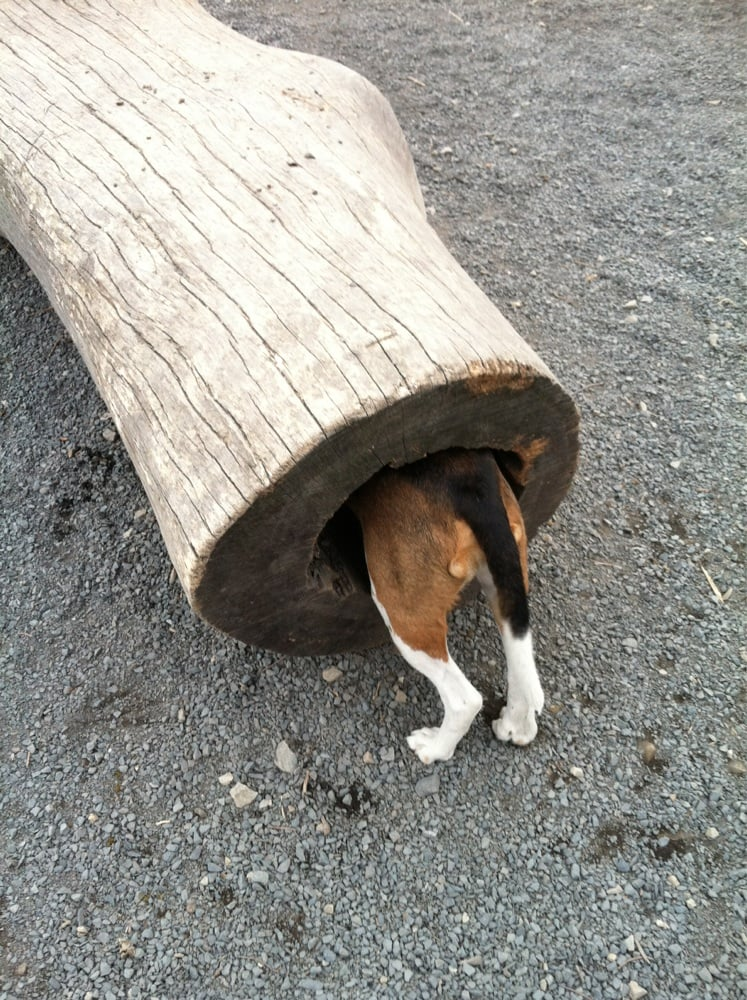
\includegraphics[scale=.2]{Lecture 7 Picture.jpg}
  \end{center}
}






\end{document}


%%% Local Variables: 
%%% mode: latex
%%% TeX-master: t
%%% End: 
